% Options for packages loaded elsewhere
\PassOptionsToPackage{unicode}{hyperref}
\PassOptionsToPackage{hyphens}{url}
%
\documentclass[
]{article}
\usepackage{amsmath,amssymb}
\usepackage{iftex}
\ifPDFTeX
  \usepackage[T1]{fontenc}
  \usepackage[utf8]{inputenc}
  \usepackage{textcomp} % provide euro and other symbols
\else % if luatex or xetex
  \usepackage{unicode-math} % this also loads fontspec
  \defaultfontfeatures{Scale=MatchLowercase}
  \defaultfontfeatures[\rmfamily]{Ligatures=TeX,Scale=1}
\fi
\usepackage{lmodern}
\ifPDFTeX\else
  % xetex/luatex font selection
\fi
% Use upquote if available, for straight quotes in verbatim environments
\IfFileExists{upquote.sty}{\usepackage{upquote}}{}
\IfFileExists{microtype.sty}{% use microtype if available
  \usepackage[]{microtype}
  \UseMicrotypeSet[protrusion]{basicmath} % disable protrusion for tt fonts
}{}
\makeatletter
\@ifundefined{KOMAClassName}{% if non-KOMA class
  \IfFileExists{parskip.sty}{%
    \usepackage{parskip}
  }{% else
    \setlength{\parindent}{0pt}
    \setlength{\parskip}{6pt plus 2pt minus 1pt}}
}{% if KOMA class
  \KOMAoptions{parskip=half}}
\makeatother
\usepackage{xcolor}
\usepackage[margin=1in]{geometry}
\usepackage{longtable,booktabs,array}
\usepackage{calc} % for calculating minipage widths
% Correct order of tables after \paragraph or \subparagraph
\usepackage{etoolbox}
\makeatletter
\patchcmd\longtable{\par}{\if@noskipsec\mbox{}\fi\par}{}{}
\makeatother
% Allow footnotes in longtable head/foot
\IfFileExists{footnotehyper.sty}{\usepackage{footnotehyper}}{\usepackage{footnote}}
\makesavenoteenv{longtable}
\usepackage{graphicx}
\makeatletter
\def\maxwidth{\ifdim\Gin@nat@width>\linewidth\linewidth\else\Gin@nat@width\fi}
\def\maxheight{\ifdim\Gin@nat@height>\textheight\textheight\else\Gin@nat@height\fi}
\makeatother
% Scale images if necessary, so that they will not overflow the page
% margins by default, and it is still possible to overwrite the defaults
% using explicit options in \includegraphics[width, height, ...]{}
\setkeys{Gin}{width=\maxwidth,height=\maxheight,keepaspectratio}
% Set default figure placement to htbp
\makeatletter
\def\fps@figure{htbp}
\makeatother
\setlength{\emergencystretch}{3em} % prevent overfull lines
\providecommand{\tightlist}{%
  \setlength{\itemsep}{0pt}\setlength{\parskip}{0pt}}
\setcounter{secnumdepth}{-\maxdimen} % remove section numbering
\ifLuaTeX
  \usepackage{selnolig}  % disable illegal ligatures
\fi
\IfFileExists{bookmark.sty}{\usepackage{bookmark}}{\usepackage{hyperref}}
\IfFileExists{xurl.sty}{\usepackage{xurl}}{} % add URL line breaks if available
\urlstyle{same}
\hypersetup{
  hidelinks,
  pdfcreator={LaTeX via pandoc}}

\author{}
\date{}

\begin{document}

\hypertarget{stentor-coeruleus-wavelength-selection-guide}{%
\section{Stentor coeruleus Wavelength Selection
Guide}\label{stentor-coeruleus-wavelength-selection-guide}}

Purpose: pool everything we've read across the \emph{S. coeruleus}
photoresponse literature into one decision --- which wavelength(s)
should StentorCam experiments prioritize to get a positive result. This
is the decision document; for general background and citation-heavy
detail (including a figure-by-figure critique of Iwatsuki 1992's axis
units and 0.58 mm/s criterion) see
\href{PHOTOKINESIS_ACTION_SPECTRUM_NOTES.md}{\texttt{PHOTOKINESIS\_ACTION\_SPECTRUM\_NOTES.md}}.
For the full experimental protocol once a wavelength is chosen (chamber
design, controls, statistics, plate layout), see
\href{ROBOCAM_ASSAY_PROTOCOL.md}{\texttt{ROBOCAM\_ASSAY\_PROTOCOL.md}},
adapted from a design document our PI provided --- it independently
reaches the same 610/620 nm recommendation and treats 680 nm as a
control wavelength, corroborating this guide.

\hypertarget{recommendation}{%
\subsection{Recommendation}\label{recommendation}}

\begin{itemize}
\tightlist
\item
  \textbf{Test 610-620 nm first.} Five independent measurements across
  three labs and 16 years (1976-1992) converge here --- the strongest,
  most replicated signal in the whole literature.
\item
  \textbf{Backup/secondary candidates: \textasciitilde560 nm and
  \textasciitilde470-480 nm.} Now corroborated by two independent papers
  (Wood 1976: 568/480 nm; Kim/Prusti/Song/Hader 1984:
  \textasciitilde555-560/470 nm) --- the same two-secondary-peak shape
  shows up twice, which is reassuring, though still lower-confidence
  than the 610-620 nm primary peak. Wood's 568 nm point was never
  directly tested in his own action spectrum (only inferred from
  absorption data); Kim/Prusti/Song/Hader's \textasciitilde555-560 nm
  point was directly measured.
\item
  \textbf{Deprioritize 680 nm.} This is Iwatsuki's claimed photokinesis
  peak, and it's an outlier by every measure we could check: single
  source, never independently replicated, no known matching pigment, and
  it's consistent with our own data showing little response there. Keep
  it as an exploratory/comparison arm, not the main bet.
\item
  \textbf{Novel angle worth pursuing regardless of the above:} none of
  the five 610-620 nm measurements were photokinesis experiments ---
  they were phototaxis or photophobic (avoidance) response. Testing
  610-620 nm specifically for \emph{photokinesis} is a measurement
  nobody has published. A positive result there would suggest
  photokinesis shares stentorin's photoreceptor rather than requiring
  Iwatsuki's proposed second, unidentified 680 nm photoreceptor.
\end{itemize}

\hypertarget{cross-paper-synthesis}{%
\subsection{Cross-paper synthesis}\label{cross-paper-synthesis}}

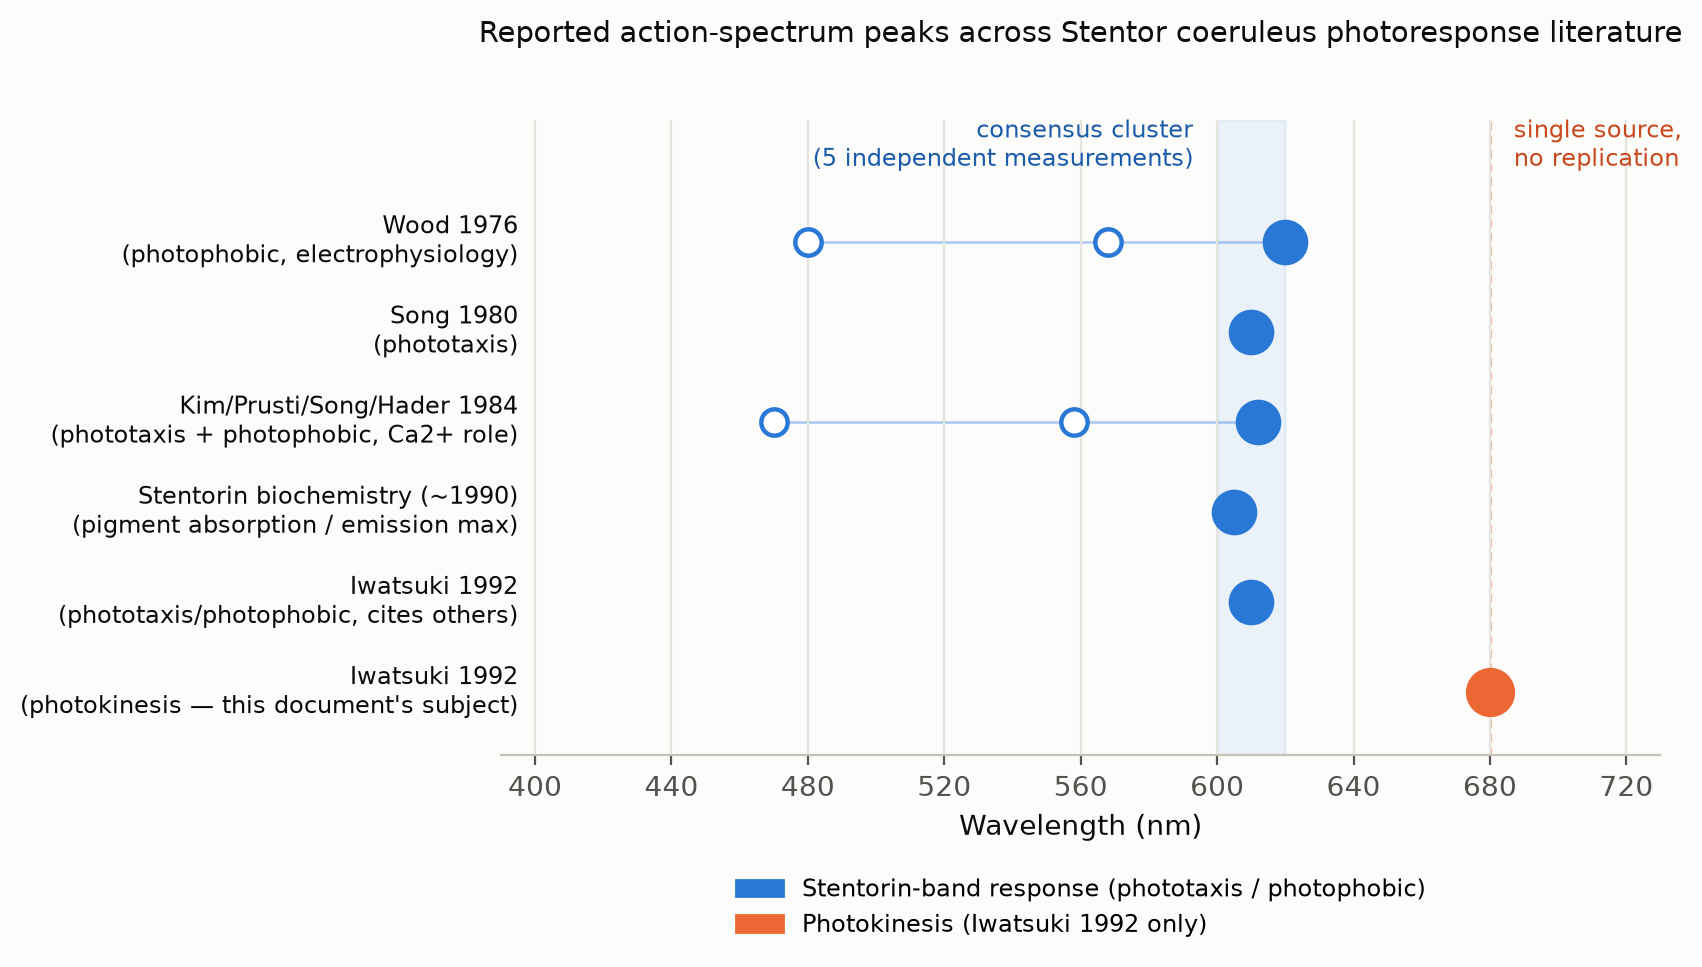
\includegraphics[width=1\textwidth,height=\textheight]{references/consensus-action-spectrum.png}

\begin{longtable}[]{@{}
  >{\raggedright\arraybackslash}p{(\columnwidth - 6\tabcolsep) * \real{0.2500}}
  >{\raggedright\arraybackslash}p{(\columnwidth - 6\tabcolsep) * \real{0.2500}}
  >{\raggedright\arraybackslash}p{(\columnwidth - 6\tabcolsep) * \real{0.2500}}
  >{\raggedright\arraybackslash}p{(\columnwidth - 6\tabcolsep) * \real{0.2500}}@{}}
\toprule\noalign{}
\begin{minipage}[b]{\linewidth}\raggedright
Source
\end{minipage} & \begin{minipage}[b]{\linewidth}\raggedright
Method
\end{minipage} & \begin{minipage}[b]{\linewidth}\raggedright
Response type
\end{minipage} & \begin{minipage}[b]{\linewidth}\raggedright
Reported peak(s)
\end{minipage} \\
\midrule\noalign{}
\endhead
\bottomrule\noalign{}
\endlastfoot
Wood 1976 & Electrophysiology + ciliary-reversal threshold & Photophobic
& 620 nm primary; 480 nm shoulder; 568 nm secondary (absorption data
only, not directly tested) \\
Song 1980 & Fluence-response curves, focused-beam orientation &
Phototaxis & \textasciitilde610 nm (broad maximum) \\
Kim/Prusti/Song/Hader 1984 & Ca2+-flux / fluence-response,
quantum-efficiency action spectrum vs.~absorption spectrum & Phototaxis
+ photophobic & \textasciitilde610-615 nm primary;
\textasciitilde555-560 nm secondary; \textasciitilde470 nm shoulder \\
Stentorin biochemistry (\textasciitilde1990, Song lab) & Absorption /
fluorescence-emission spectroscopy of the isolated pigment & Pigment
characterization & \textasciitilde600-620 nm \\
Iwatsuki 1992 & Fluence-response curves (cites the above) &
Phototaxis/photophobic & 610 nm \\
\textbf{Iwatsuki 1992} & Fluence-response curves, criterion velocity &
\textbf{Photokinesis} & \textbf{680 nm --- the outlier} \\
\end{longtable}

Wood 1976, Song 1980, and Kim/Prusti/Song/Hader 1984 values above are
confirmed directly from the primary-source PDFs (now in
\texttt{references/}) --- the ILL request for Kim/Prusti/Song/Hader came
through. Its Fig. 1 plots a proper quantum-efficiency action spectrum
directly against stentorin's measured absorption spectrum (in vivo and
at 77 K), and its multi-peak shape (\textasciitilde610-615 nm primary,
\textasciitilde555-560 nm secondary, \textasciitilde470 nm shoulder)
independently reproduces Wood 1976's pattern (620/568/480 nm) almost
exactly --- two separate labs, two different methods (fluence-rate
criterion-response vs. direct quantum-efficiency calculation),
converging on the same multi-band shape. That's a much stronger
corroboration of the 610-620 nm cluster than a single-paper result. Only
the stentorin-biochemistry summary is still from a secondary source
pending full-text access.

The photoreceptor behind the 610-620 nm cluster is identified:
\textbf{stentorin}, a hypericin-based chromophore with absorption
confined to roughly 525-630 nm. It has essentially no absorption at 680
nm --- which is exactly why Iwatsuki had to propose a second, distinct
photoreceptor system to explain the photokinesis result. No follow-up
work in the 30+ years since has identified what that second
photoreceptor might be, and \emph{S. coeruleus} has no
plastids/chlorophyll that would otherwise explain red-region sensitivity
out at 680 nm.

\hypertarget{why-680-nm-specifically-looks-weak-summary}{%
\subsection{Why 680 nm specifically looks weak
(summary)}\label{why-680-nm-specifically-looks-weak-summary}}

\begin{itemize}
\tightlist
\item
  \textbf{Single source.} Of 24+ papers citing Iwatsuki (1992), none
  independently re-measured the photokinesis action spectrum --- all
  just cite it as background.
\item
  \textbf{No replication attempt succeeded.} Kühnel-Kratz \& Häder
  (1994) is the one paper that re-examined photokinesis behavior with
  improved 3D tracking, but they used white light only --- no
  monochromatic wavelength sweep --- so it neither confirms nor refutes
  680 nm.
\item
  \textbf{No matching pigment.} See above.
\item
  \textbf{Thin derivation of the criterion response.} Iwatsuki's action
  spectrum is built by finding the fluence rate needed to hit a fixed
  criterion velocity (0.58 mm/s) at each wavelength; the paper doesn't
  explain why 0.58 mm/s specifically, beyond it being a value within the
  overlapping range of all nine tested curves. (Full breakdown in
  \texttt{PHOTOKINESIS\_ACTION\_SPECTRUM\_NOTES.md}.)
\end{itemize}

\hypertarget{other-experimental-variables-to-control-for}{%
\subsection{Other experimental variables to control
for}\label{other-experimental-variables-to-control-for}}

\begin{itemize}
\tightlist
\item
  \textbf{Fluence-rate ceiling.} Kühnel-Kratz \& Häder (1994) only saw
  positive photokinesis below \textasciitilde10 W/m\^{}2; above that, no
  clear kinesis --- in tension with Iwatsuki's claim of an almost-linear
  velocity-vs-log-fluence relationship across the \emph{entire} tested
  range. Check where our fluence rates fall relative to this cutoff.
\item
  \textbf{Chamber geometry.} Kühnel-Kratz \& Häder's dark-swimming
  baseline velocities (1.5-1.8 mm/s) were notably higher than every
  previously published value (0.2-1.2 mm/s, including Iwatsuki's),
  attributed to their wider 25 mm cuvette reducing wall effects. Our own
  baseline velocities may not be directly comparable to the literature
  unless our chamber width/depth is accounted for.
\item
  \textbf{Light-source spectral purity.} Confirm actual output spectrum
  at whichever wavelength setting we test (LED/filter bandwidth can
  shift or wash out a narrow real peak) --- relevant whether we're
  testing 610-620 nm or 680 nm.
\end{itemize}

\hypertarget{light-sources-what-the-papers-used-vs.-our-apparatus}{%
\subsection{Light sources: what the papers used vs.~our
apparatus}\label{light-sources-what-the-papers-used-vs.-our-apparatus}}

\textbf{What the classic papers actually used} (confirmed from the
primary-source PDFs, now all in \texttt{references/}) --- none used
lasers or LEDs; all were filtered lamp/projector setups:

\begin{longtable}[]{@{}
  >{\raggedright\arraybackslash}p{(\columnwidth - 4\tabcolsep) * \real{0.3333}}
  >{\raggedright\arraybackslash}p{(\columnwidth - 4\tabcolsep) * \real{0.3333}}
  >{\raggedright\arraybackslash}p{(\columnwidth - 4\tabcolsep) * \real{0.3333}}@{}}
\toprule\noalign{}
\begin{minipage}[b]{\linewidth}\raggedright
Paper
\end{minipage} & \begin{minipage}[b]{\linewidth}\raggedright
Light source
\end{minipage} & \begin{minipage}[b]{\linewidth}\raggedright
Wavelength selection
\end{minipage} \\
\midrule\noalign{}
\endhead
\bottomrule\noalign{}
\endlastfoot
Iwatsuki 1992 & Incandescent lamp, IR cut-off filter + water container &
Interference filter (\textless6 nm half-bandwidth) + neutral-density
filters; EG\&G photometer \\
Wood 1976 & Zircon arc lamp (behavioral test); cool white fluorescent
bulbs (electrophysiology test) & Interference filters, 10 nm
half-bandwidth, stepped every 20 nm 480-660 nm; ND + heat filters \\
Song 1980 & 40 W incandescent lamp, collimated & ND filters (white
light); interference filters (Baird Atomic, \textasciitilde10 nm
half-bandwidth); Kettering Model 65 radiometer \\
Kim/Prusti/Song/Hader 1984 & 300 W slide projector (Gold) & Interference
filters, \textasciitilde10 nm half-bandwidth; Kettering Y.S.I. Model 65A
radiant power meter \\
Kuhnel-Kratz \& Hader 1994 & 15 W Zeiss microscope lamp (viewing); 150 W
halogen (Schott KL 1500 / Osram Xenophot, stimulus) & White light only
--- no wavelength filtering, consistent with them never testing an
action spectrum \\
\end{longtable}

\textbf{Our apparatus:} the plotting scripts
(\texttt{full\_data\_plot.py}, \texttt{track\_plot.py}) label the
stimulus ``LED On''/``LED Off'' in their legends, even though the
README's CLI flags are loosely named after ``laser color'' --- that's
historical naming, not a hardware spec, and no BOM/part number for
either an LED or a laser diode exists in this repo (hardware specifics
live in the separate RoboCam repo).

\textbf{Current build direction: a laser-based coaxial illuminator with
a 50/50 beamsplitter}, sharing the optical axis with the camera. For
that specific design, a laser diode is the better fit optically (small
collimated beam couples through a beamsplitter far more efficiently than
an LED, which needs extra collimating optics and loses more power to
etendue mismatch). Recommended source: a \textbf{\textasciitilde605-620
nm orange laser diode module} --- this wavelength sits in what's called
the semiconductor ``yellow-orange gap'' (570-625 nm is hard for direct
diode lasers), so it's a specialty part rather than an off-the-shelf
pointer diode, but real products exist (RPMC Lasers' 590-619 nm orange
category, Laserland's 600-640 nm modules, Thorlabs' visible laser diode
line). A common 635 nm red diode is the cheap fallback, but Wood 1976's
own data shows ``a large decrease\ldots{} between 620 and 640 nm,'' so
expect a weaker response than a true 605-620 nm source. For the 480 nm
and 680 nm arms, standard blue (\textasciitilde450-473 nm) and deep-red
(\textasciitilde650-685 nm) diodes are cheap and common --- no gap issue
there.

To get a \textbf{consistent, uniform spot covering a well (6-20 mm
diameter) over a 0.5-2 ft throw}: collimate the diode, then pass it
through a fixed Galilean beam expander (e.g.~Thorlabs GBE, 5x on a
\textasciitilde3 mm collimated beam gives \textasciitilde15 mm output)
to hold the spot size steady across that distance range, then an
engineered diffuser (e.g.~Thorlabs ED1-C series) to flatten the Gaussian
profile into a top-hat so every point in the well gets the same fluence
rate. An iris/aperture after the diffuser can clip to an exact diameter
within the 6-20 mm target if needed. Keep total power modest ---
Iwatsuki's tested range was \textasciitilde0.1-1.1 W/m\^{}2, and
Kuhnel-Kratz \& Hader saw kinesis disappear above \textasciitilde10
W/m\^{}2 --- a few mW, attenuated by driver current or an ND filter, is
plenty.

\hypertarget{suggested-next-experiment-design}{%
\subsection{Suggested next-experiment
design}\label{suggested-next-experiment-design}}

\begin{enumerate}
\def\labelenumi{\arabic{enumi}.}
\tightlist
\item
  Primary arm: \textbf{610 nm and 620 nm}, measuring photokinesis
  (swimming velocity), not just avoidance/phototaxis.
\item
  Secondary arms: \textbf{480 nm and 568 nm} as backup candidates.
\item
  Comparison arm: \textbf{680 nm}, kept in the design specifically to
  directly test Iwatsuki's claim against our own setup, now that we know
  it's an unreplicated outlier rather than settled fact.
\item
  Keep fluence rates under \textasciitilde10 W/m\^{}2 per the
  Kühnel-Kratz ceiling, and record chamber width/depth so results are
  comparable across studies.
\item
  If 610-620 nm produces a clear photokinesis response, that's a novel
  result (nobody has published a photokinesis measurement at that
  wavelength) supporting a shared photoreceptor with the
  phototaxis/photophobic response. If it doesn't, that keeps the
  second-photoreceptor question open --- but 680 nm still wouldn't be
  confirmed by our data either, so a positive result there would itself
  be noteworthy given the literature gap.
\end{enumerate}

\hypertarget{source-status}{%
\subsection{Source status}\label{source-status}}

\begin{longtable}[]{@{}
  >{\raggedright\arraybackslash}p{(\columnwidth - 2\tabcolsep) * \real{0.5000}}
  >{\raggedright\arraybackslash}p{(\columnwidth - 2\tabcolsep) * \real{0.5000}}@{}}
\toprule\noalign{}
\begin{minipage}[b]{\linewidth}\raggedright
Paper
\end{minipage} & \begin{minipage}[b]{\linewidth}\raggedright
Status
\end{minipage} \\
\midrule\noalign{}
\endhead
\bottomrule\noalign{}
\endlastfoot
Iwatsuki 1992 & Local reference library (not committed --- copyright),
values verified \\
Wood 1976 & Local reference library (not committed --- copyright),
values verified \\
Song 1980 & Local reference library (not committed --- copyright),
values verified \\
Kuhnel-Kratz \& Hader 1994 & Local reference library (not committed ---
copyright), read --- no wavelength data \\
Kim/Prusti/Song/Hader 1984 & Local reference library (not committed ---
copyright, ILL came through), values verified \\
\end{longtable}

Full-text PDFs for all five papers above are kept outside this repo (in
a local reference library) rather than committed. Wood 1976, Song 1980,
Kim/Prusti/Song/Hader 1984, and Kuhnel-Kratz \& Hader 1994 came with ILL
cover sheets with an explicit ``no further copies, electronic or paper''
restriction that doesn't permit redistribution. Iwatsuki 1992's PDF has
no such cover-sheet notice, but it's still a copyrighted journal article
--- it was committed to this repo and pushed to the public fork earlier
in this project before this concern came up; that commit has since been
removed from history and force-pushed, and the PDF moved to the same
local reference library as the others. Every value we cite from all five
papers has been independently re-verified against the primary-source PDF
text before being written into these docs, even though the PDFs
themselves live outside the repo. The derived Figure 3 crop image
(\texttt{references/iwatsuki-1992-figure3-action-spectrum.png}) is still
committed, since it's a small excerpt used for commentary/critique
rather than the full paper.

\end{document}
